\documentclass{article}
\usepackage{tikz}

\begin{document}

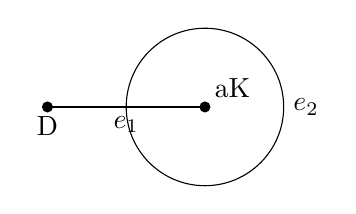
\begin{tikzpicture}[scale=1]
    % Draw the circle
    \draw (0,0) circle (1);
    
    % Draw the line segment
    \draw (-2,0) -- (0,0);
    
    % Label the points and distances
    \fill (-2,0) circle (2pt) node[below] {D};
    \fill (0,0) circle (2pt) node[above right] {aK};
    \node at (-1,0) [below] {$e_1$};
    \node at (1,0) [right] {$e_2$};
\end{tikzpicture}

\end{document}